\chapter{Experimental Results}
\label{chap:results}

This chapter compares throughput at measured recall, analyzes the effect of
\(N_{\mathrm{list}}\) and \(N_{\mathrm{probe}}\), decomposes the Tenstorrent
search path, and reports workload energy. Throughput is the median of ten
search-only repetitions, whereas energy covers the complete 100,000-query
session of Equation~\ref{eq:queries-per-run}, including initialization.

\section{CPU, GPU, and Tenstorrent Comparison}
\label{sec:cross-platform-performance}

Figure~\ref{fig:qps-recall} shows QPS against measured Recall@10 on a
logarithmic throughput axis. Placing recall rather than
\(N_{\mathrm{probe}}\) on the horizontal axis allows the Tenstorrent
batch-union implementation to be compared with per-query IVF search without
assuming equivalent candidate sets. Table~\ref{tab:qps-matched} extracts the
four recall-matched operating points of Table~\ref{tab:recall-matched-points}.

\begin{figure}[htbp]
\centering
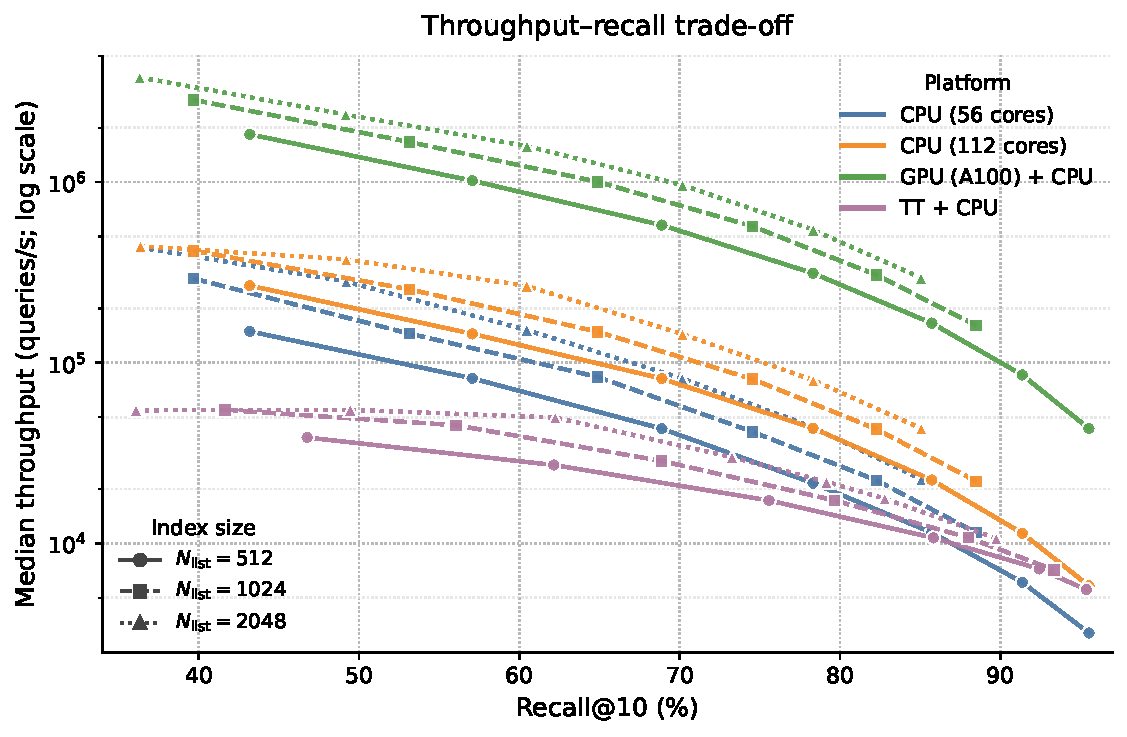
\includegraphics[width=0.94\textwidth]{./assets/qps_vs_recall.pdf}
\caption{Queries per second versus measured Recall@10. Each point is the median
of ten repetitions, and lines connect \(N_{\mathrm{probe}}\) values within one
\(N_{\mathrm{list}}\) sweep. The Tenstorrent \((2048,12)\) energy-matching point
is included; other exploratory \(N_{\mathrm{probe}}=12\) runs are not.}
\label{fig:qps-recall}
\end{figure}

\begin{table}[htbp]
\centering
\caption{Median search throughput at the recall-matched operating points of
Table~\ref{tab:recall-matched-points}. The ratio is baseline QPS divided by
Tenstorrent QPS, so values above one favor the baseline.}
\label{tab:qps-matched}
\small
\setlength{\tabcolsep}{4pt}
\renewcommand{\arraystretch}{1.08}
\begin{tabular}{lrrrrrrr}
\toprule
& \multicolumn{4}{c}{Median QPS} & \multicolumn{3}{c}{Ratio to TT} \\
\cmidrule(lr){2-5}\cmidrule(lr){6-8}
Target & CPU (56) & CPU (112) & A100 & TT & CPU (56) & CPU (112) & A100 \\
\midrule
60\% & 151,858 & 266,184 & 1,583,712 & 49,720 & 3.05 & 5.35 & 31.85 \\
78\% & 43,864  & 80,075  & 544,703   & 21,907 & 2.00 & 3.66 & 24.86 \\
88\% & 11,466  & 22,079  & 160,799   & 10,762 & 1.07 & 2.05 & 14.94 \\
95\% & 3,190   & 5,822   & 43,271    & 5,550  & 0.57 & 1.05 & 7.80 \\
\bottomrule
\end{tabular}
\end{table}

The GPU is the fastest configuration across the whole recall range, by a
factor of 31.9 over Tenstorrent at the 60\% target and 7.8 at the 95\% target.
Tenstorrent is also slower than both CPU configurations up to about 88\%
recall: the 56-core CPU is 3.05 times faster at 60\% and reaches parity at
88\%, while the 112-core CPU remains 2.05 times faster at 88\%. The crossover
with the 56-core CPU lies near 90\% recall: Tenstorrent at \((512,16)\) reaches
92.4\% recall at 7,229~QPS, whereas the CPU reaches 91.4\% at 6,090~QPS with
\((512,32)\). At the 95\% target, Tenstorrent is 1.74 times faster than the
56-core CPU and within 5\% of the 112-core CPU. These comparisons hold against
the evaluated grid: near 95\% recall the only Faiss point is \((512,64)\),
whereas Section~\ref{sec:nlist-nprobe-results} shows that Faiss is faster with
more lists, so configurations with more lists and larger
\(N_{\mathrm{probe}}\), which were not evaluated, could narrow or reverse the
CPU comparison. Within the evaluated grid, Tenstorrent's relative position
improves steadily with recall, because its throughput falls more
slowly than that of the baselines as search depth grows. When
\(N_{\mathrm{probe}}\) doubles, Faiss scans twice as many lists for every
query, and its throughput roughly halves: at 512 lists, going from
\(N_{\mathrm{probe}}=16\) to 32 lowers it by a factor of 1.89 on the 56-core
CPU. On Tenstorrent, the work per batch is set by the union of the lists
selected by its queries, and the additional lists increasingly overlap with
those already selected by other queries, so the union grows by much less than
a factor of two (Section~\ref{sec:nlist-nprobe-results}). At 512 lists, its
pages grow by a factor of 1.51 from \(N_{\mathrm{probe}}=8\) to 16 and of 1.31
from 16 to 32, and the throughput falls by almost the same factors, 1.49 and
1.30. At low recall, however, Tenstorrent is limited by a fixed per-batch cost,
also analyzed in Section~\ref{sec:nlist-nprobe-results}.

The 112-core CPU is faster than the 56-core CPU at every configuration, but
the speed-up depends on the amount of work per query. It is small when little
candidate work is available, only 1.02 at \((2048,1)\), 1.33 at
\((2048,2)\), and 1.42 at \((1024,1)\), because per-call overheads then
dominate. With more work it
lies between 1.75 and 2.01 without a monotonic trend, peaking at \((512,8)\).
Near-linear and occasionally slightly super-linear scaling is consistent with
the larger aggregate cache and memory bandwidth available to the full node.

Run-to-run variation is small compared with the differences between
platforms. Across the complete grid, the QPS RSD of
Equation~\ref{eq:qps-rsd} is at most 4.64\% for the 56-core CPU, 5.89\% for
the 112-core CPU, 2.43\% for the GPU, and 1.46\% for Tenstorrent, and the
ten repetitions show no systematic first-repetition slowdown. The medians in
Figure~\ref{fig:qps-recall} and Table~\ref{tab:qps-matched} are therefore
not driven by individual repetitions.

\section{Impact of \texorpdfstring{\(N_{\mathrm{list}}\) and
\(N_{\mathrm{probe}}\)}{Nlist and Nprobe}}
\label{sec:nlist-nprobe-results}

Within every sweep, increasing \(N_{\mathrm{probe}}\) raises recall and lowers
throughput. The choice of \(N_{\mathrm{list}}\), however, affects the platforms
differently.

\paragraph{Faiss favors finer partitions.}
At matched recall, the Faiss baselines are faster with more lists. Near 78\%
recall, the GPU reaches 544,703~QPS at \((2048,16)\) but only 313,161~QPS at
\((512,8)\), a factor of 1.74; the gain is 2.03 on the 56-core CPU and 1.84 on the
112-core CPU.
Smaller lists reduce the candidate volume per probe more than the larger
coarse scan costs.

\paragraph{The batch union raises Tenstorrent recall.}
Table~\ref{tab:union-recall-gain} compares Tenstorrent and Faiss recall at the
same configuration. Because every query is also scored against lists selected
by other queries in its batch, Tenstorrent is more accurate at almost every
point, by up to 7.52 percentage points at \((512,8)\). The gain first grows
with \(N_{\mathrm{probe}}\) and then shrinks as recall approaches saturation.
It also decreases with \(N_{\mathrm{list}}\): the maximum is 7.52 points for
512 lists, 5.74 for 1024, and 4.67 for 2048. This is consistent with lists
contributed by other queries being less likely to contain a query's true
neighbors when the partition is finer.

\begin{table}[htbp]
\centering
\caption{Recall@10 difference, Tenstorrent minus Faiss CPU, in percentage
points at equal \((N_{\mathrm{list}},N_{\mathrm{probe}})\).}
\label{tab:union-recall-gain}
\small
\setlength{\tabcolsep}{6pt}
\renewcommand{\arraystretch}{1.08}
\begin{tabular}{lrrrrrr}
\toprule
& \multicolumn{6}{c}{\(N_{\mathrm{probe}}\)} \\
\cmidrule(lr){2-7}
\(N_{\mathrm{list}}\) & 1 & 2 & 4 & 8 & 16 & 32 \\
\midrule
512  & \(+3.58\) & \(+5.08\) & \(+6.68\) & \(+7.52\) & \(+6.71\) & \(+4.00\) \\
1024 & \(+1.95\) & \(+2.89\) & \(+4.00\) & \(+5.12\) & \(+5.74\) & \(+4.85\) \\
2048 & \(-0.27\) & \(+0.25\) & \(+1.78\) & \(+3.10\) & \(+4.46\) & \(+4.67\) \\
\bottomrule
\end{tabular}
\end{table}

\paragraph{The union multiplies the scanned data.}
The recall gain has a cost. Figure~\ref{fig:union-scanned-fraction} and
Table~\ref{tab:union-scan} compare the fraction of the database against which
each query is scored on Tenstorrent, whose queries scan the whole batch union,
with the fraction that Faiss scans through the query's own
\(N_{\mathrm{probe}}\) lists. Both use the lists selected by the Tenstorrent
coarse search, logged on the host for one repetition of 10,000 queries; the
batching is deterministic, and a repeated run produced identical unions. At
equal parameters, a Tenstorrent query is scored against 12 to 32 times as many
vectors as a Faiss query. At the four energy operating points it scans 6.7\%,
18.3\%, 41.0\%, and 81.7\% of the database, so at the 95\% target the fine
search is close to an exhaustive scan.

\begin{figure}[htbp]
\centering
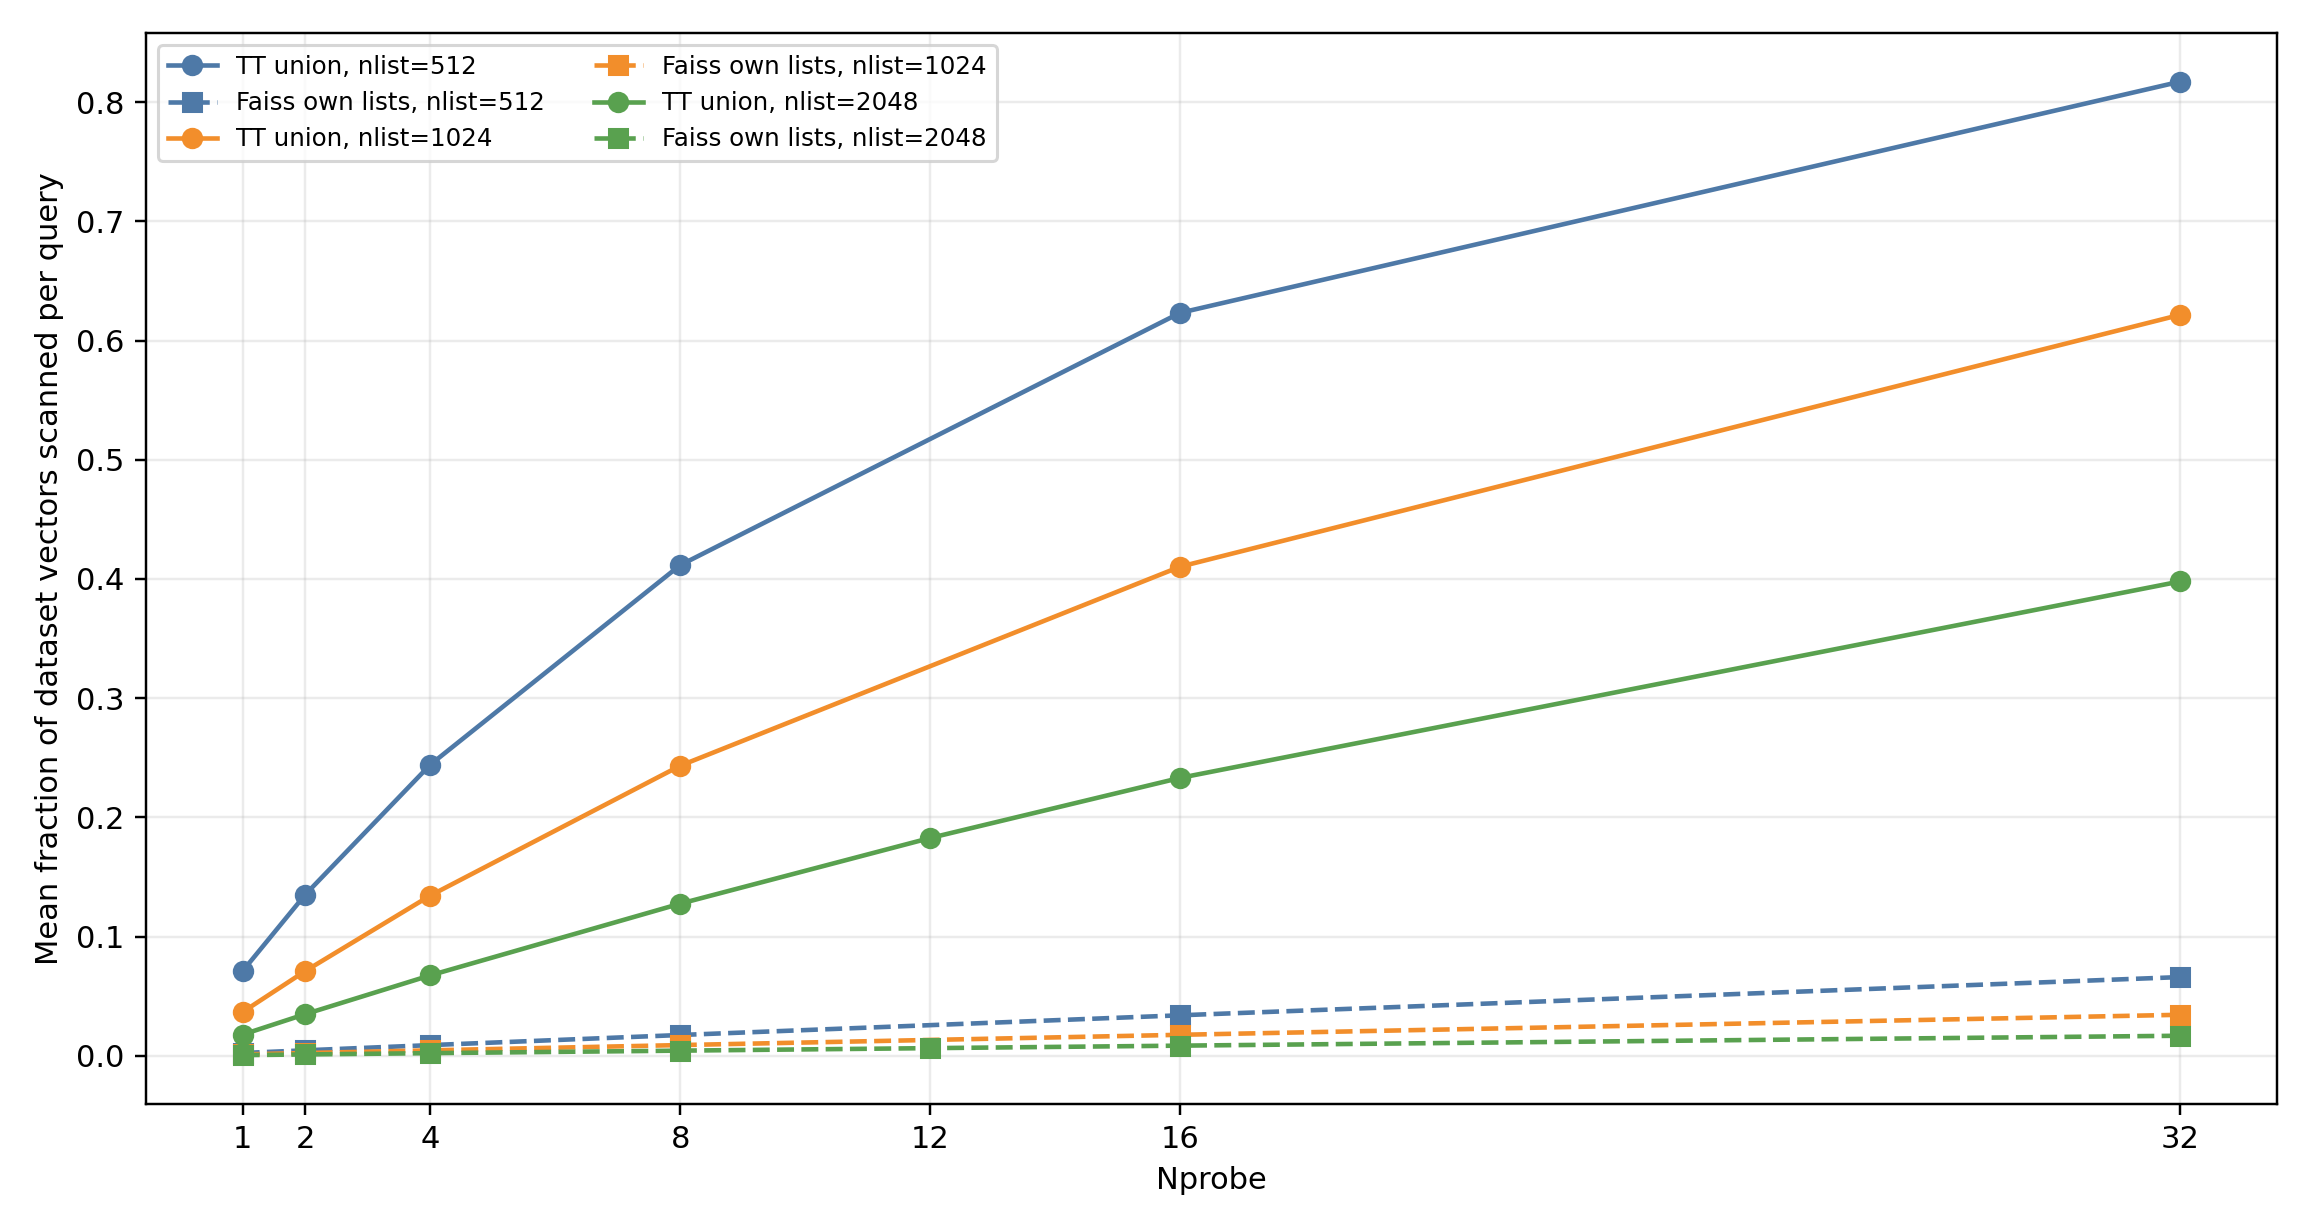
\includegraphics[width=0.94\textwidth]{./assets/union_scanned_fraction.png}
\caption{Mean fraction of the database scanned per query as a function of
\(N_{\mathrm{probe}}\): the batch union on Tenstorrent (solid) and the query's
own lists as in Faiss (dashed), for each \(N_{\mathrm{list}}\).}
\label{fig:union-scanned-fraction}
\end{figure}

\begin{table}[htbp]
\centering
\caption{Mean fraction of the database scanned per query on Tenstorrent, and
the factor by which it exceeds the vectors in the query's own
\(N_{\mathrm{probe}}\) lists. A factor of 32 means that the 32 queries of a
batch share no lists.}
\label{tab:union-scan}
\small
\setlength{\tabcolsep}{5pt}
\renewcommand{\arraystretch}{1.08}
\begin{tabular}{llrrrrrrr}
\toprule
& & \multicolumn{7}{c}{\(N_{\mathrm{probe}}\)} \\
\cmidrule(lr){3-9}
\(N_{\mathrm{list}}\) & & 1 & 2 & 4 & 8 & 12 & 16 & 32 \\
\midrule
512  & scanned & 7.1\% & 13.5\% & 24.4\% & 41.1\% & -- & 62.3\% & 81.7\% \\
     & factor  & 30.6 & 29.5 & 27.3 & 23.6 & -- & 18.3 & 12.4 \\
\midrule
1024 & scanned & 3.7\% & 7.1\% & 13.4\% & 24.3\% & -- & 41.0\% & 62.1\% \\
     & factor  & 31.2 & 30.6 & 29.4 & 27.1 & -- & 23.3 & 18.1 \\
\midrule
2048 & scanned & 1.8\% & 3.5\% & 6.7\% & 12.8\% & 18.3\% & 23.3\% & 39.8\% \\
     & factor  & 31.6 & 31.3 & 30.7 & 29.6 & 28.5 & 27.4 & 23.7 \\
\bottomrule
\end{tabular}
\end{table}

The factors close to 32 show that consecutive queries in dataset order share
almost no lists. At \((2048,4)\), for example, the 128 lists requested by a
batch contain a median of 124 distinct lists. Overlap appears only when the
union covers a large part of all lists, as at \((512,32)\), where 1,024
selections contain a median of 412 distinct lists, or 80\% of the 512. This
explains the recall gain of Table~\ref{tab:union-recall-gain}, which is bought
with a much larger scan, and why the gain falls with finer partitions, where
each extra list covers a smaller part of the database. It also explains why
Tenstorrent's position against the CPUs improves with recall: its scanned
volume approaches the whole database and grows slowly, whereas the per-query
scan of Faiss keeps growing with \(N_{\mathrm{probe}}\).

The union is nevertheless the right choice for the device. Every query must
still be scored against its own \(N_{\mathrm{probe}}\) lists, and each
fine-search step multiplies a full 32-query tile regardless of how many rows
are useful. Processing the queries separately would therefore fetch and
multiply every selected list once per query that requests it, whereas the
union fetches each distinct list only once per batch. The number of pages
fetched falls by the overlap factor, the ratio of requested to distinct lists,
and the extra candidates that each query receives come from lists fetched for
other queries at no additional matrix multiplication. In dataset order,
however, the overlap factor is only 1.0--2.5, so the saving is small; grouping
queries that select similar lists into the same batch would raise it.

\paragraph{Tenstorrent sweeps converge at high recall.}
Above about 85\% recall, the three Tenstorrent sweeps nearly coincide:
\((512,8)\), \((1024,16)\), and \((2048,32)\) all run at about 10,700~QPS and
reach 85.83\%, 88.03\%, and 89.75\% recall respectively. In this regime
\(N_{\mathrm{list}}\) mainly shifts recall at similar cost, and 2048 lists give
the best trade-off.

\paragraph{Tenstorrent has a fixed per-batch floor.}
At low \(N_{\mathrm{probe}}\), Tenstorrent throughput stops increasing:
\((1024,1)\), \((2048,1)\), and \((2048,2)\) all run at about 54,800~QPS, or
about 182~ms per 10,000 queries, even though their candidate volumes differ.
This corresponds to roughly 0.58~ms per 32-query batch that does not depend on
\(N_{\mathrm{probe}}\). At 2048 lists the most likely cause is the final
aggregation. The
aggregation core processes the batches one after another, and for every batch
it merges one top-32 result from each of the 63 workers, including workers
without assigned lists (Section~\ref{subsec:hierarchical-topk}). In the batch
trace of Section~\ref{subsec:tt-device-timeline-results} this takes about
0.44~ms per batch, close to the floor. At larger \(N_{\mathrm{probe}}\) the
workers need several milliseconds per batch, so the aggregation overlaps with
their work and is not a bottleneck; at low \(N_{\mathrm{probe}}\) the workers
finish a batch sooner than the aggregation, which then becomes a likely
bottleneck. This floor caps Tenstorrent's low-recall throughput and explains
much of its gap to the CPUs at the 60\% target. Load imbalance contributes as
well: at \(N_{\mathrm{probe}}=1\) a batch union holds at most 32 lists, so at
most 32 of the 63 workers can receive work, and in the logged schedule, which
does not split lists, the busiest worker holds a median of 3.7--4.2 times the
mean load; at 1024 lists this imbalance alone may account for most of the
floor. The stage decomposition below covers only
\(N_{\mathrm{list}}=512\), where candidate work dominates, so it does not
isolate this cost.

\section{Tenstorrent Stage Decomposition}
\label{sec:tt-stage-results}

Figure~\ref{fig:tt-stage-full} shows the six stages of
Equation~\ref{eq:tt-stage-sum-method} for \(N_{\mathrm{list}}=512\) and
\(N_{\mathrm{probe}}\in\{1,8,16,32\}\). Each segment is the median of that stage
over ten repetitions of 10,000 queries, after one warm-up invocation, so a
stack height is a sum of
stage-wise medians. Figure~\ref{fig:tt-stage-detail} omits TT fine search and
rescales the vertical axis to expose the remaining stages.

\begin{figure}[htbp]
\centering
\begin{minipage}[t]{0.49\textwidth}
\centering
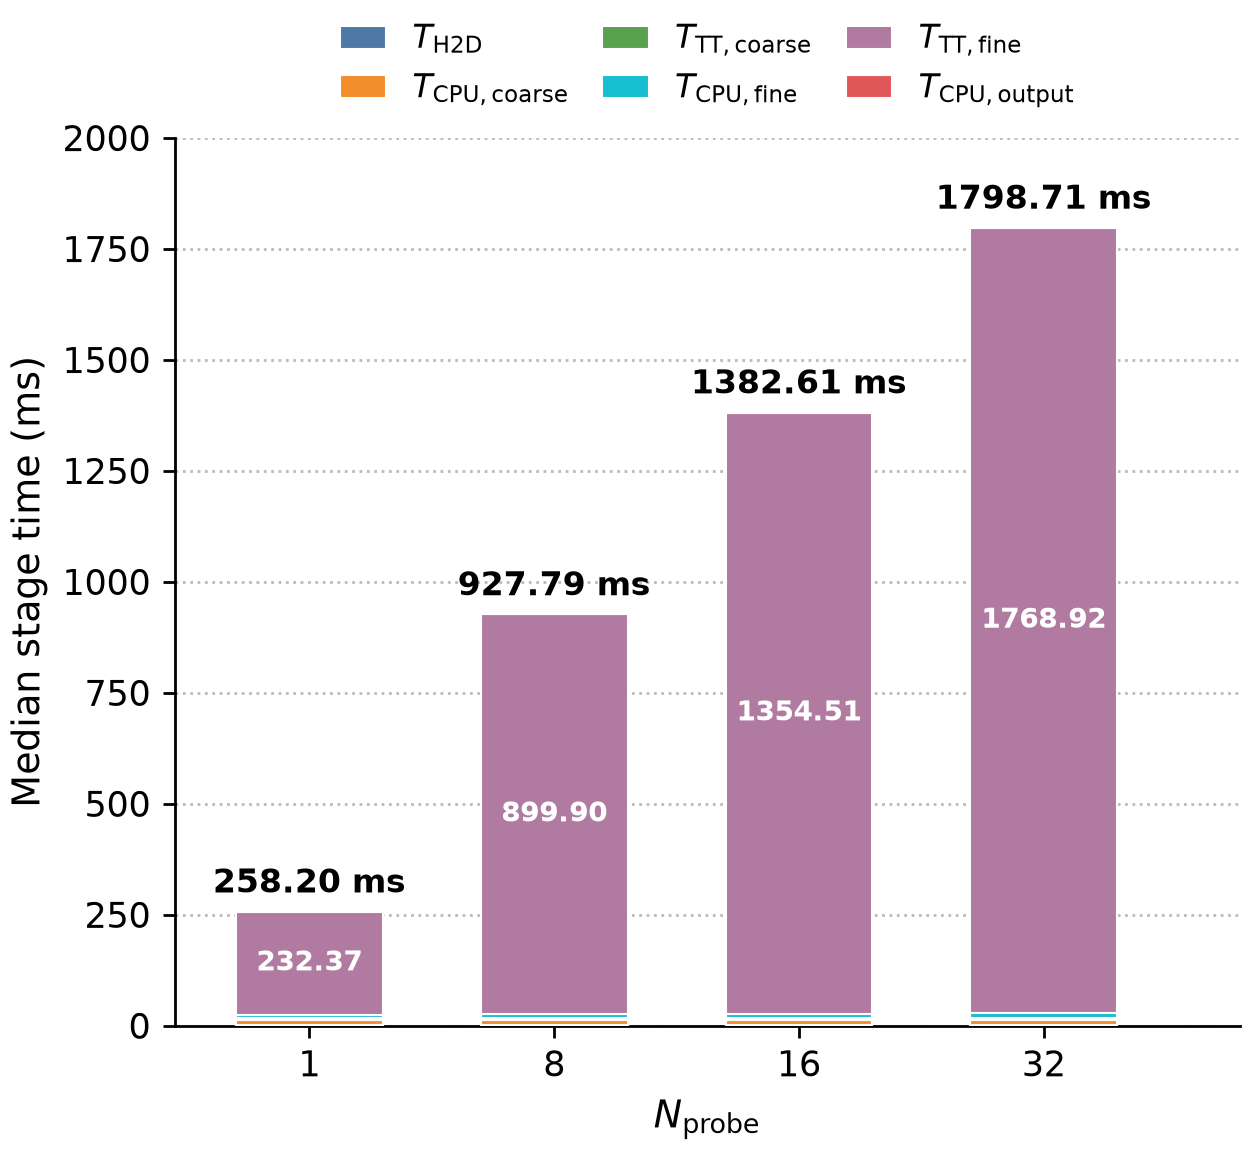
\includegraphics[width=\textwidth]
{./assets/memcopy_cost_nlist512.png}
\caption{Median Tenstorrent stage times for \(N_{\mathrm{list}}=512\),
including TT fine search.}
\label{fig:tt-stage-full}
\end{minipage}
\hfill
\begin{minipage}[t]{0.49\textwidth}
\centering
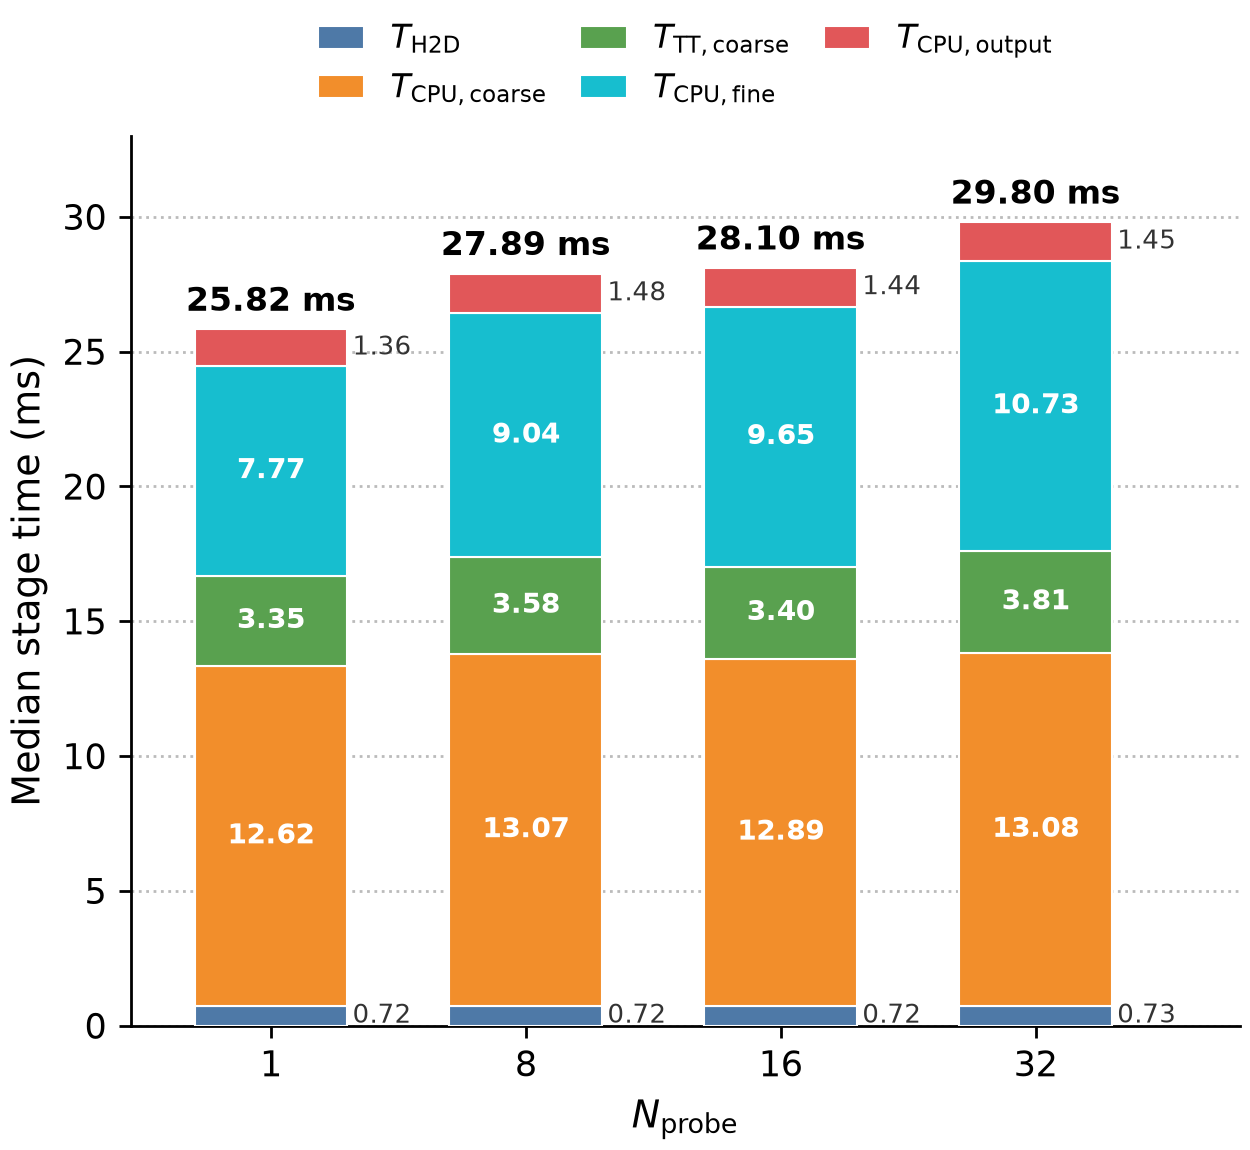
\includegraphics[width=\textwidth]
{./assets/memcopy_cost_nlist512_without_tt_fine.png}
\caption{Rescaled view of the same stage times with TT fine search omitted.}
\label{fig:tt-stage-detail}
\end{minipage}
\end{figure}

TT fine search dominates. As \(N_{\mathrm{probe}}\) increases from 1 to 32, the
total rises from 258.20 to 1,798.71~ms and fine search from 232.37 to
1,768.92~ms, accounting for 90.0\%, 97.0\%, 98.0\%, and 98.3\% of the four
totals. The totals agree with the independent throughput measurements: 1,798.71~ms
per 10,000 queries corresponds to about 5,560~QPS, against a median of 5,550~QPS.
All other stages together grow only from 25.82 to 29.80~ms: CPU coarse
configuration stays between 12.62 and 13.08~ms, TT coarse search between 3.35
and 3.81~ms, and CPU fine preparation grows from 7.77 to 10.73~ms. Optimizing
these stages would therefore have little effect at this \(N_{\mathrm{list}}\).
Host timing cannot tell whether compute, DRAM traffic, NoC communication,
circular-buffer backpressure, or synchronization limits the fine stage, which
motivates the device trace below.

\subsection{Device-Kernel Timeline}
\label{subsec:tt-device-timeline-results}

Figure~\ref{fig:tt-fine-pipeline-zoom} shows a device-profiler capture with
\(N_{\mathrm{list}}=512\) and \(N_{\mathrm{probe}}=8\), which reaches 85.8\%
recall, zoomed into the last three measured batches, labeled B1 to B3. It
covers the aggregation core and three consecutive fine-search workers. The
workers were taken in coordinate order, not selected by behavior, so the
figure is illustrative rather than a statistical sample of all workers. The
figure separates each core into its reader (NCRISC) and its three
compute threads (TRISC unpack, math, and pack). Each
worker scope is labeled with its batch and list task, so a bar covers the
processing of one task: a complete list or a chunk of at most 128 pages.

\begin{figure}[htbp]
\centering
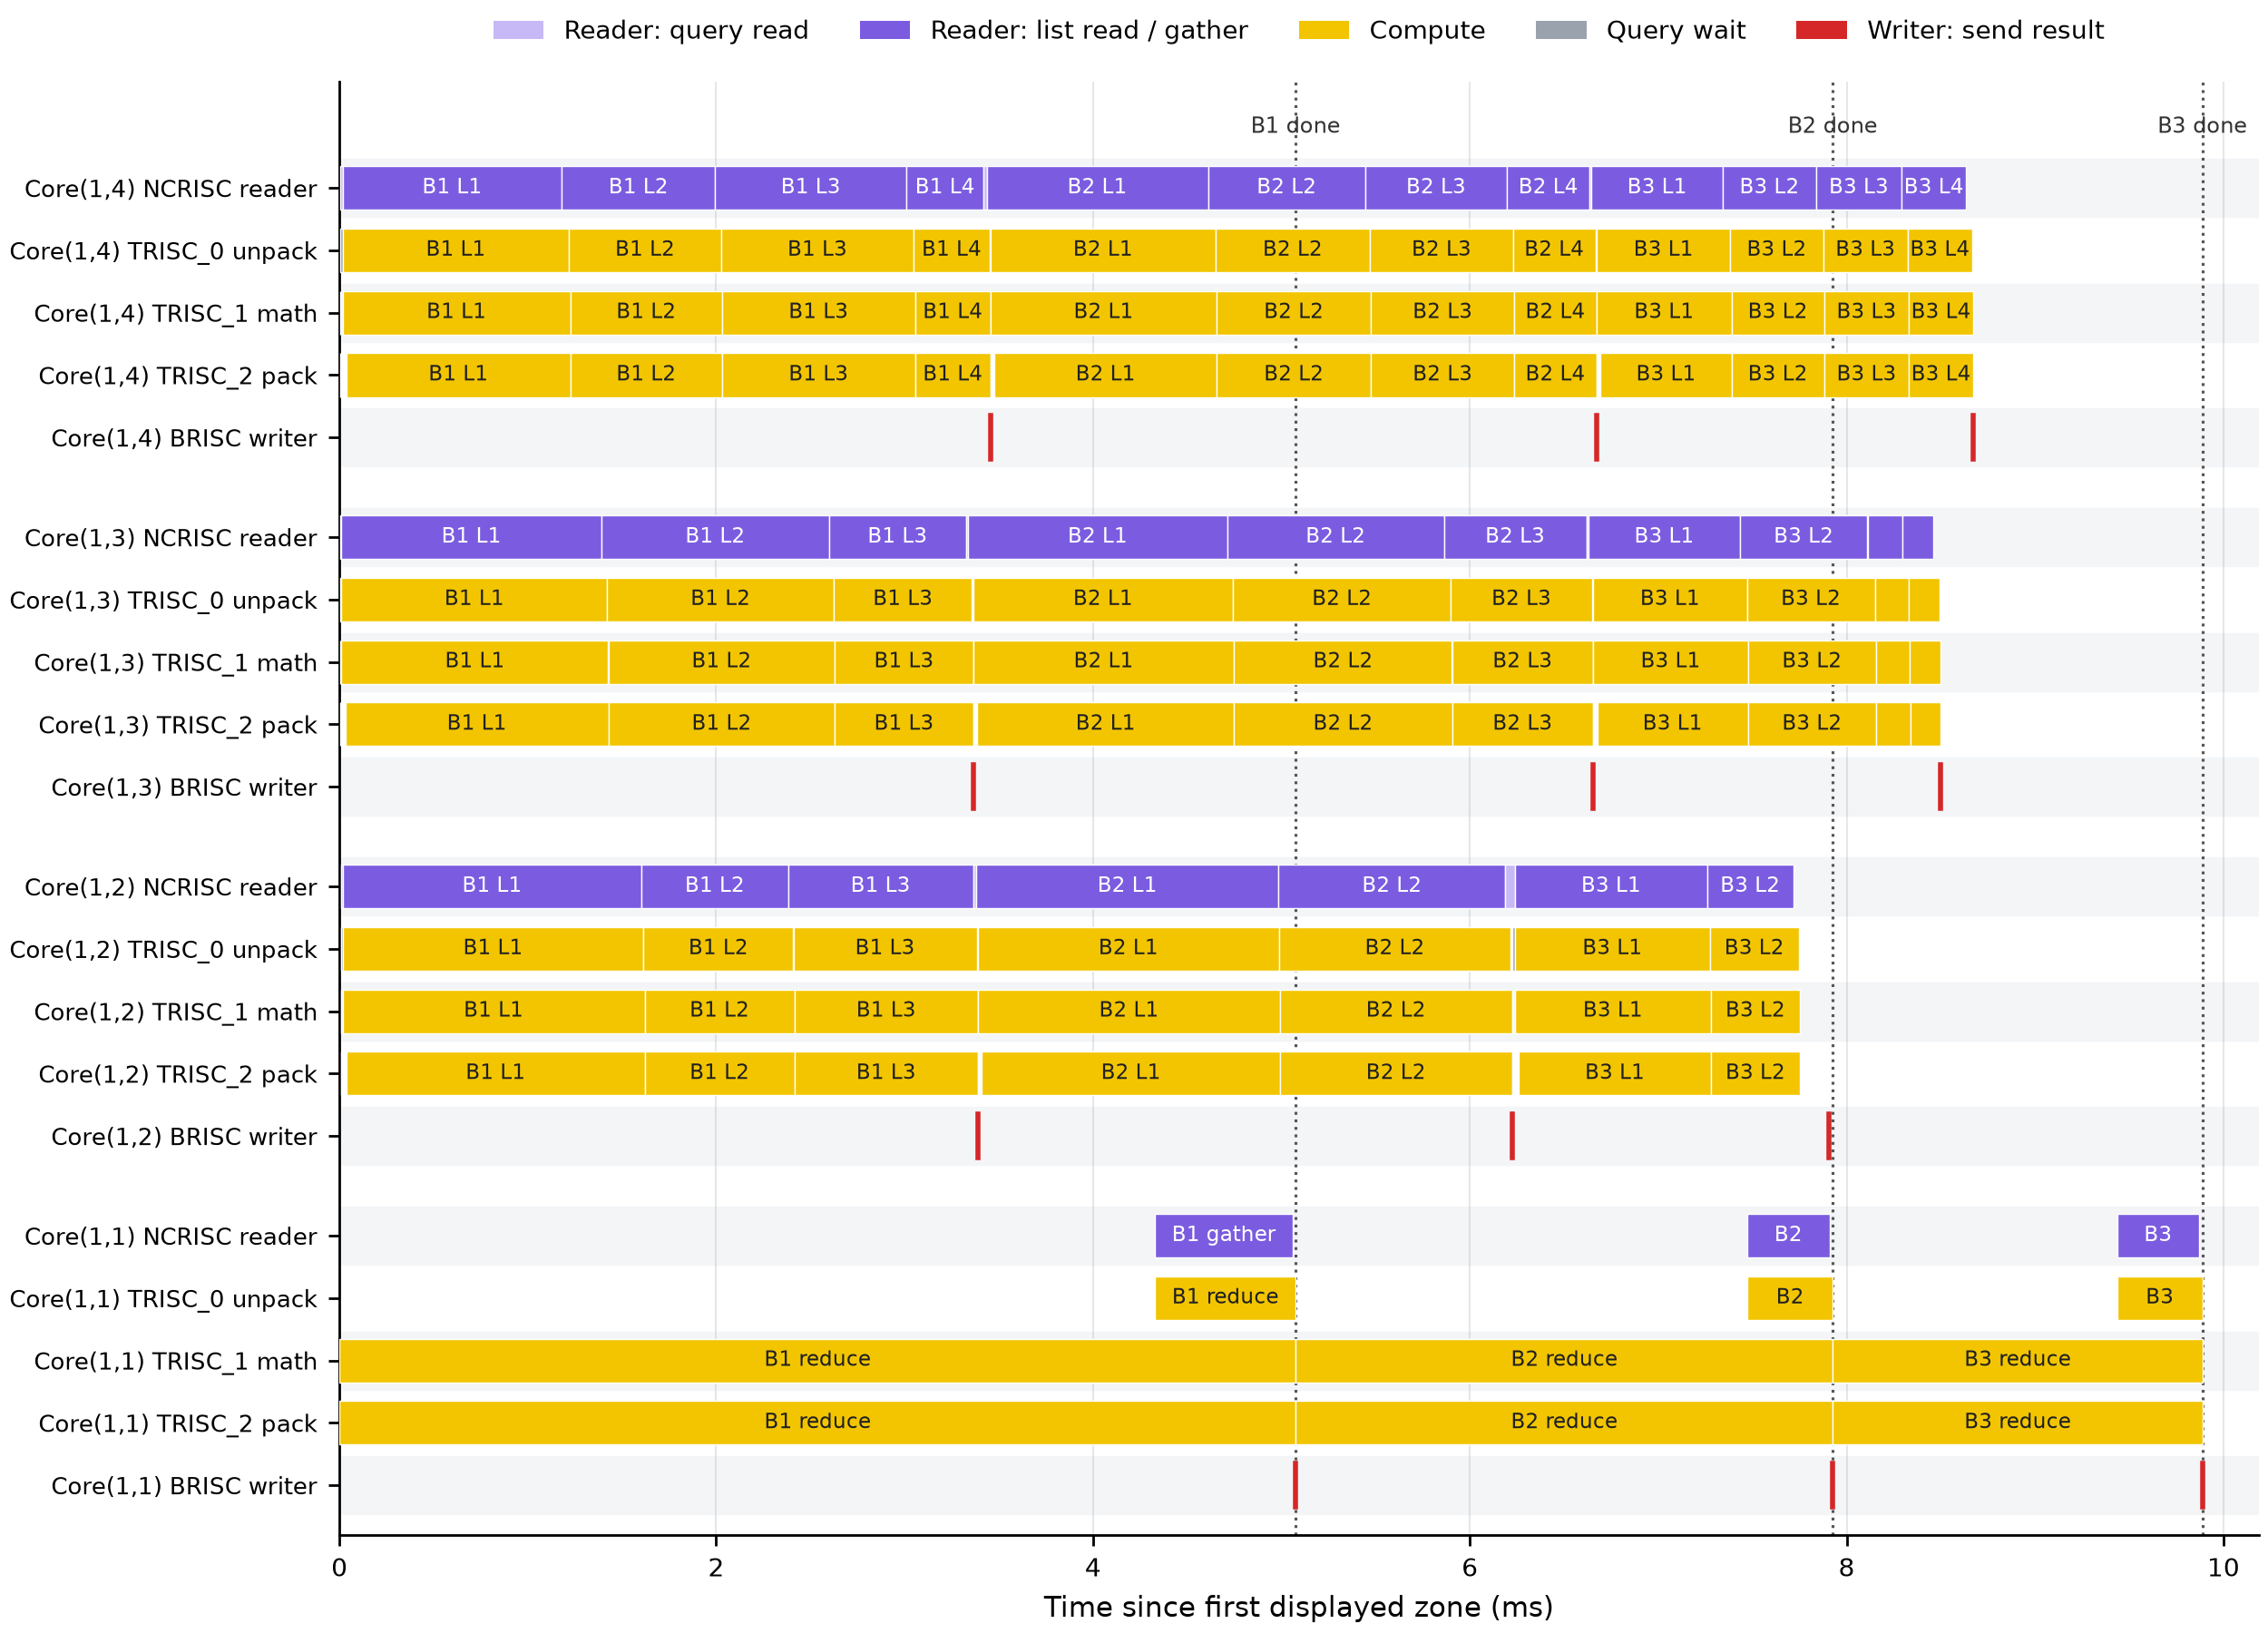
\includegraphics[width=\textwidth,keepaspectratio]
{./assets/fine_pipeline_horizontal.png}
\caption{Zoomed fine-search pipeline at
\((N_{\mathrm{list}},N_{\mathrm{probe}})=(512,8)\) for the last three 32-query
batches (B1 to B3), with one row per RISC processor of the aggregation core
(profiler core \((1,1)\)) and of three workers (profiler cores \((1,2)\) to
\((1,4)\)). A worker zone labeled B\(b\) L\(i\) covers the \(i\)-th list
task of batch \(b\); red ticks mark the writer sending a result, and dotted
lines mark the completion of each batch on the aggregation core.}
\label{fig:tt-fine-pipeline-zoom}
\end{figure}

Four observations follow from the zoomed trace.

\begin{enumerate}
    \item \textbf{Workers do not stop between batches.} Each worker starts the
    first list of the next batch within a few tens of microseconds of finishing
    the previous one. The aggregation core gathers B1 between about 4.3 and
    5.1~ms, when the three workers shown are already processing B2. Batch
    reduction is therefore off the workers' critical path and introduces no
    per-batch barrier.
    \item \textbf{Reader and compute advance in lock-step.} On every worker,
    each reader scope ends a few tens of microseconds before the corresponding
    compute scope, and the unpack, math, and pack scopes coincide. The
    pipeline overlaps the reading and scoring of the same list, and its fill
    latency at the start of a batch is only about 30--40~\(\mu\)s. Because each
    scope spans a whole task, the trace still cannot tell whether compute
    waits for data or the reader is throttled by full circular buffers.
    \item \textbf{Worker imbalance sets batch completion.} The three workers
    finish B1 within about 0.1~ms of each other, but drift apart later,
    completing B3 at about 7.8, 8.5, and 8.7~ms. The aggregator's B1 gather
    starts about 0.9~ms after the last of the three workers shown has finished
    B1, which is consistent with other workers finishing later. As batch
    completion depends on the slowest of the 63 workers, the greedy
    assignment of coarse list tasks translates directly into idle
    capacity.
    \item \textbf{Aggregation is short and overlapped.} The aggregator's
    gather and unpack scopes last about 0.73, 0.44, and 0.44~ms for the three
    batches. Its math and pack scopes span almost the entire interval because
    they include waiting for worker results, not because reduction is
    expensive. At this configuration the aggregation is therefore not an
    issue, but at low \(N_{\mathrm{probe}}\), where the workers finish a
    batch faster, the same per-batch cost becomes a likely bottleneck
    (Section~\ref{sec:nlist-nprobe-results}).
\end{enumerate}

The 2.85~ms between the completions of B1 and B2 matches the 2.96~ms per
batch measured by the stage timing at this configuration (927.79~ms over 313
batches), so the zoomed batches are representative. Batch B3 is visibly shorter on all workers because it is the final batch of
the repetition, which holds only 16 valid queries
(Equation~\ref{eq:tt-batches-per-repetition}) and therefore a smaller list
union. Each worker's writer sends its fixed-size local result in under
1~\(\mu\)s per batch, shown as red ticks.

Overall, the zoomed trace shows that fine-search time is spent inside the
per-list reader--compute loop of each worker and is extended by imbalance
across workers, whereas batch transitions and aggregation contribute little.

\paragraph{Single-list zoom.}
Figure~\ref{fig:tt-fine-cluster-bubbles} zooms further, into the processing of
16 consecutive pages (P0 to P15) of one inverted list on worker \((1,2)\),
captured with
\(N_{\mathrm{list}}=512\) and \(N_{\mathrm{probe}}=1\). Reader zones cover the
DRAM fetch of each page, and compute zones cover the unpacking, scoring, and
top-\(k\) update of each page.

\begin{figure}[htbp]
\centering
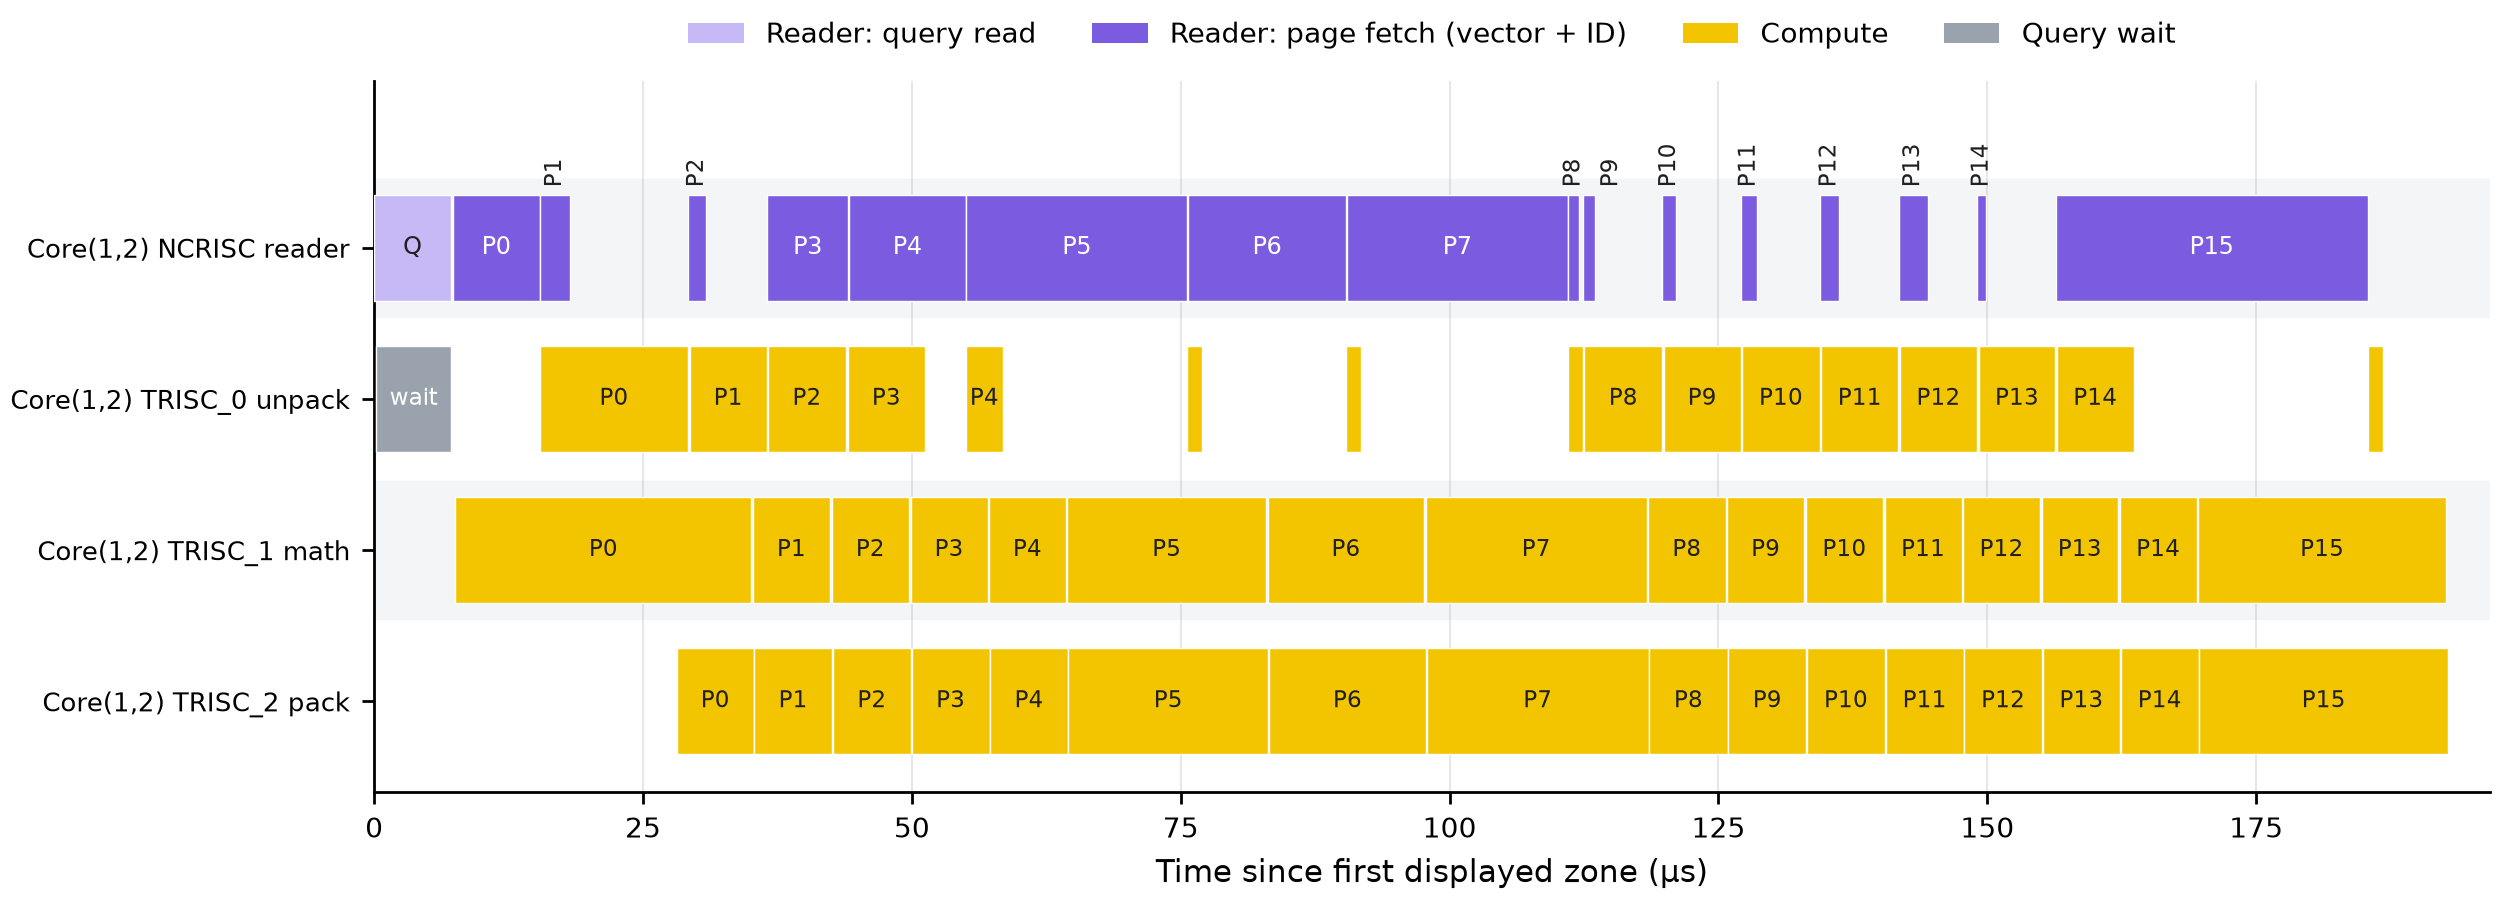
\includegraphics[width=\textwidth,keepaspectratio]
{./assets/fine_cluster_bubbles.png}
\caption{Processing of 16 consecutive pages (P0 to P15) of one inverted list on worker
\((1,2)\) at \((N_{\mathrm{list}},N_{\mathrm{probe}})=(512,1)\). The reader row
shows the query fetch and the DRAM fetch of each page; the compute rows show
the work on each page and the initial wait for the query.}
\label{fig:tt-fine-cluster-bubbles}
\end{figure}

\begin{enumerate}
    \item \textbf{Compute costs about 7~\(\mu\)s per page.} When data is
    available (P1 to P4 and P8 to P14), each page occupies the math and pack
    threads for about 7~\(\mu\)s, while the reader fetches the next
    page mostly in under 3~\(\mu\)s shortly before it is needed. In this regime
    the pipeline is limited by the per-page compute step, not by arithmetic
    (see below), and the reader waits for free buffer space. A
    page requires only four \(32\times32\) tile multiplications, so the
    7~\(\mu\)s suggests that most of the compute time is spent outside the
    matrix multiplication, in the top-\(k\) update.
    \item \textbf{Slow fetches create bubbles.} The fetches of P5, P6, P7, and
    P15 take 15--29~\(\mu\)s instead of under 3~\(\mu\)s. The unpacker then has no
    input, and the math and pack zones of these pages stretch to
    15--23~\(\mu\)s. Start-up adds a further bubble: the query fetch and the
    first page read delay the pack thread until about 28~\(\mu\)s, and the
    first page is complete only at about 35~\(\mu\)s.
    \item \textbf{About 40\% of the time is waiting.} Sixteen pages at
    about 7~\(\mu\)s account for roughly 115~\(\mu\)s of the 193~\(\mu\)s
    shown, so compute waits for data for about 40\% of the time.
    \item \textbf{The buffer hides little variation.} The reader runs only
    about one page ahead of compute, as expected from the double-buffered
    candidate buffers (Section~\ref{subsec:fine-worker-pipeline}), so a
    single slow fetch stalls the
    pipeline immediately, whereas the 8--11~\(\mu\)s fetches of P3 and P4 are
    hidden because they start early enough. Deeper buffering does not solve
    this, however: in single exploratory runs at \((512,32)\) with an
    instrumented build, letting the reader prefetch eight pages instead of two
    made fine search about 7\% slower (2,006 against 1,880~ms per 10,000
    queries), consistent with the additional outstanding reads adding to the
    contention between workers for the DRAM channels.
\end{enumerate}

\paragraph{Arithmetic intensity.} The ``compute'' in the trace is not
arithmetic. Each page fetches 12,288~bytes, 8,192 for the 32 vectors of 128
FP16 dimensions and 4,096 for the identifier tile, and performs one
\(32\times128\) by \(128\times32\) multiplication of 262,144 floating-point
operations. Even with all 32 query rows in use, this is only 21~operations per
byte, an order of magnitude below the balance point of the Wormhole n150, about
257~operations per byte for its 74~FP16 TFLOP/s and 288~GB/s
\cite{tenstorrent_wormhole_spec}. Most rows are not even useful: only the
queries that selected the list need its scores, which on average is one row
in 12 to 31 (Table~\ref{tab:union-scan}), so the useful intensity is only
0.7--1.7~operations per byte. The fine search is therefore memory-bound in the
roofline sense, and the matrix engine is never its limit: at \((512,32)\) it
runs at about 1.4~TFLOP/s, 2\% of the peak. The DRAM is not saturated either,
since the 9.5~million pages fetched in 1.77~s amount to about 66~GB/s, 23\% of
the peak bandwidth. The time per page is set instead by the work around the
multiplication, chiefly the top-\(k\) update of the scores and identifiers, and
by the latency of the fetches, which become slow and irregular when many
workers read at the same time. Both depend on the number of pages processed,
which is why reducing that number matters more than faster arithmetic.

\paragraph{Growth with \(N_{\mathrm{probe}}\).}
The window was captured at \(N_{\mathrm{probe}}=1\), which is the most
favorable case for data availability: the union of a 32-query batch then
contains at most 32 lists, so at most 32 of the 63 workers are active. Three
effects are expected to enlarge the problem as \(N_{\mathrm{probe}}\) grows.
\begin{enumerate}
    \item \textbf{More concurrent readers.} From \(N_{\mathrm{probe}}=2\)
    onwards, the union can exceed the 63 workers, so all of them fetch pages
    at the same time and compete for the same DRAM channels and NoC links.
    The trace does not show why the fetches of P5 to P7 and P15 are slow, but
    if contention is the cause, such fetches become more frequent and longer.
    \item \textbf{More pages per worker.} Each worker processes more list
    tasks per batch, so every stall is repeated over more pages. Even at an
    unchanged fraction of waiting per page, the absolute waiting time grows
    with the number of pages scanned.
    \item \textbf{Constant compute cost per page.} The approximately
    7~\(\mu\)s per page does not decrease with \(N_{\mathrm{probe}}\), so the
    phases limited by the per-page compute step also grow in proportion to
    the pages scanned.
\end{enumerate}
Consistently with these effects, TT fine search grows from 232 to
1,769~ms per 10,000 queries between \(N_{\mathrm{probe}}=1\) and 32
(Section~\ref{sec:tt-stage-results}).
Reducing the data fetched per query and the cost of the per-page top-\(k\)
update are the two main directions for improving fine search.

\section{Workload Energy}
\label{sec:energy-results}

Table~\ref{tab:energy-recall} and Figure~\ref{fig:query-energy} report the
median energy of ten complete 100,000-query sessions at each recall-matched
point, amortized per query with Equation~\ref{eq:energy-per-query}, together
with the interquartile range (IQR) and the relative standard deviation (RSD)
across the ten sessions. For Tenstorrent, the energy is that of the complete
system, device and host together.

\begin{table}[htbp]
\centering
\caption{Workload energy for 100,000-query sessions, including
initialization. Energy is the median of ten sessions, with the IQR and RSD
across them, and its amortized per-query value. Configuration denotes
\((N_{\mathrm{list}},N_{\mathrm{probe}})\).}
\label{tab:energy-recall}
\small
\setlength{\tabcolsep}{2.4pt}
\renewcommand{\arraystretch}{1.08}
\begin{tabular}{lrrrrrr}
\toprule
Architecture & Config. & Recall@10 & Energy (J) & IQR (J) & RSD & mJ/query \\
\midrule
CPU (56 cores)  & \((2048,4)\)  & 60.46\% & 6,995.69  & 6,927--7,090   & 2.36\% & 69.957 \\
                & \((2048,16)\) & 78.33\% & 7,981.57  & 7,901--8,070   & 1.93\% & 79.816 \\
                & \((1024,32)\) & 88.49\% & 9,211.55  & 9,140--9,351   & 1.40\% & 92.116 \\
                & \((512,64)\)  & 95.54\% & 21,872.36 & 21,831--21,988 & 0.67\% & 218.724 \\
\midrule
CPU (112 cores) & \((2048,4)\)  & 60.46\% & 6,915.42  & 6,835--7,002   & 2.65\% & 69.154 \\
                & \((2048,16)\) & 78.33\% & 7,526.78  & 7,467--7,747   & 2.67\% & 75.268 \\
                & \((1024,32)\) & 88.49\% & 7,292.36  & 7,270--7,371   & 1.50\% & 72.924 \\
                & \((512,64)\)  & 95.54\% & 14,928.76 & 14,741--15,060 & 1.46\% & 149.288 \\
\midrule
GPU (A100) + CPU & \((2048,4)\)  & 60.47\% & 932.97   & 776--1,085   & 36.60\% & 9.330 \\
                 & \((2048,16)\) & 78.33\% & 940.54   & 847--1,019   & 24.01\% & 9.405 \\
                 & \((1024,32)\) & 88.49\% & 1,064.14 & 1,021--1,113 & 5.72\%  & 10.641 \\
                 & \((512,64)\)  & 95.53\% & 2,010.66 & 1,989--2,131 & 6.23\%  & 20.107 \\
\midrule
TT + CPU         & \((2048,4)\)  & 62.24\% & 3,050.09 & 3,036--3,076 & 1.78\% & 30.501 \\
                 & \((2048,12)\) & 79.16\% & 3,542.92 & 3,525--3,562 & 3.85\% & 35.429 \\
                 & \((1024,16)\) & 88.03\% & 3,438.38 & 3,420--3,457 & 1.32\% & 34.384 \\
                 & \((512,32)\)  & 95.37\% & 4,692.64 & 4,669--4,741 & 1.93\% & 46.926 \\
\bottomrule
\end{tabular}
\end{table}

\begin{figure}[htbp]
\centering
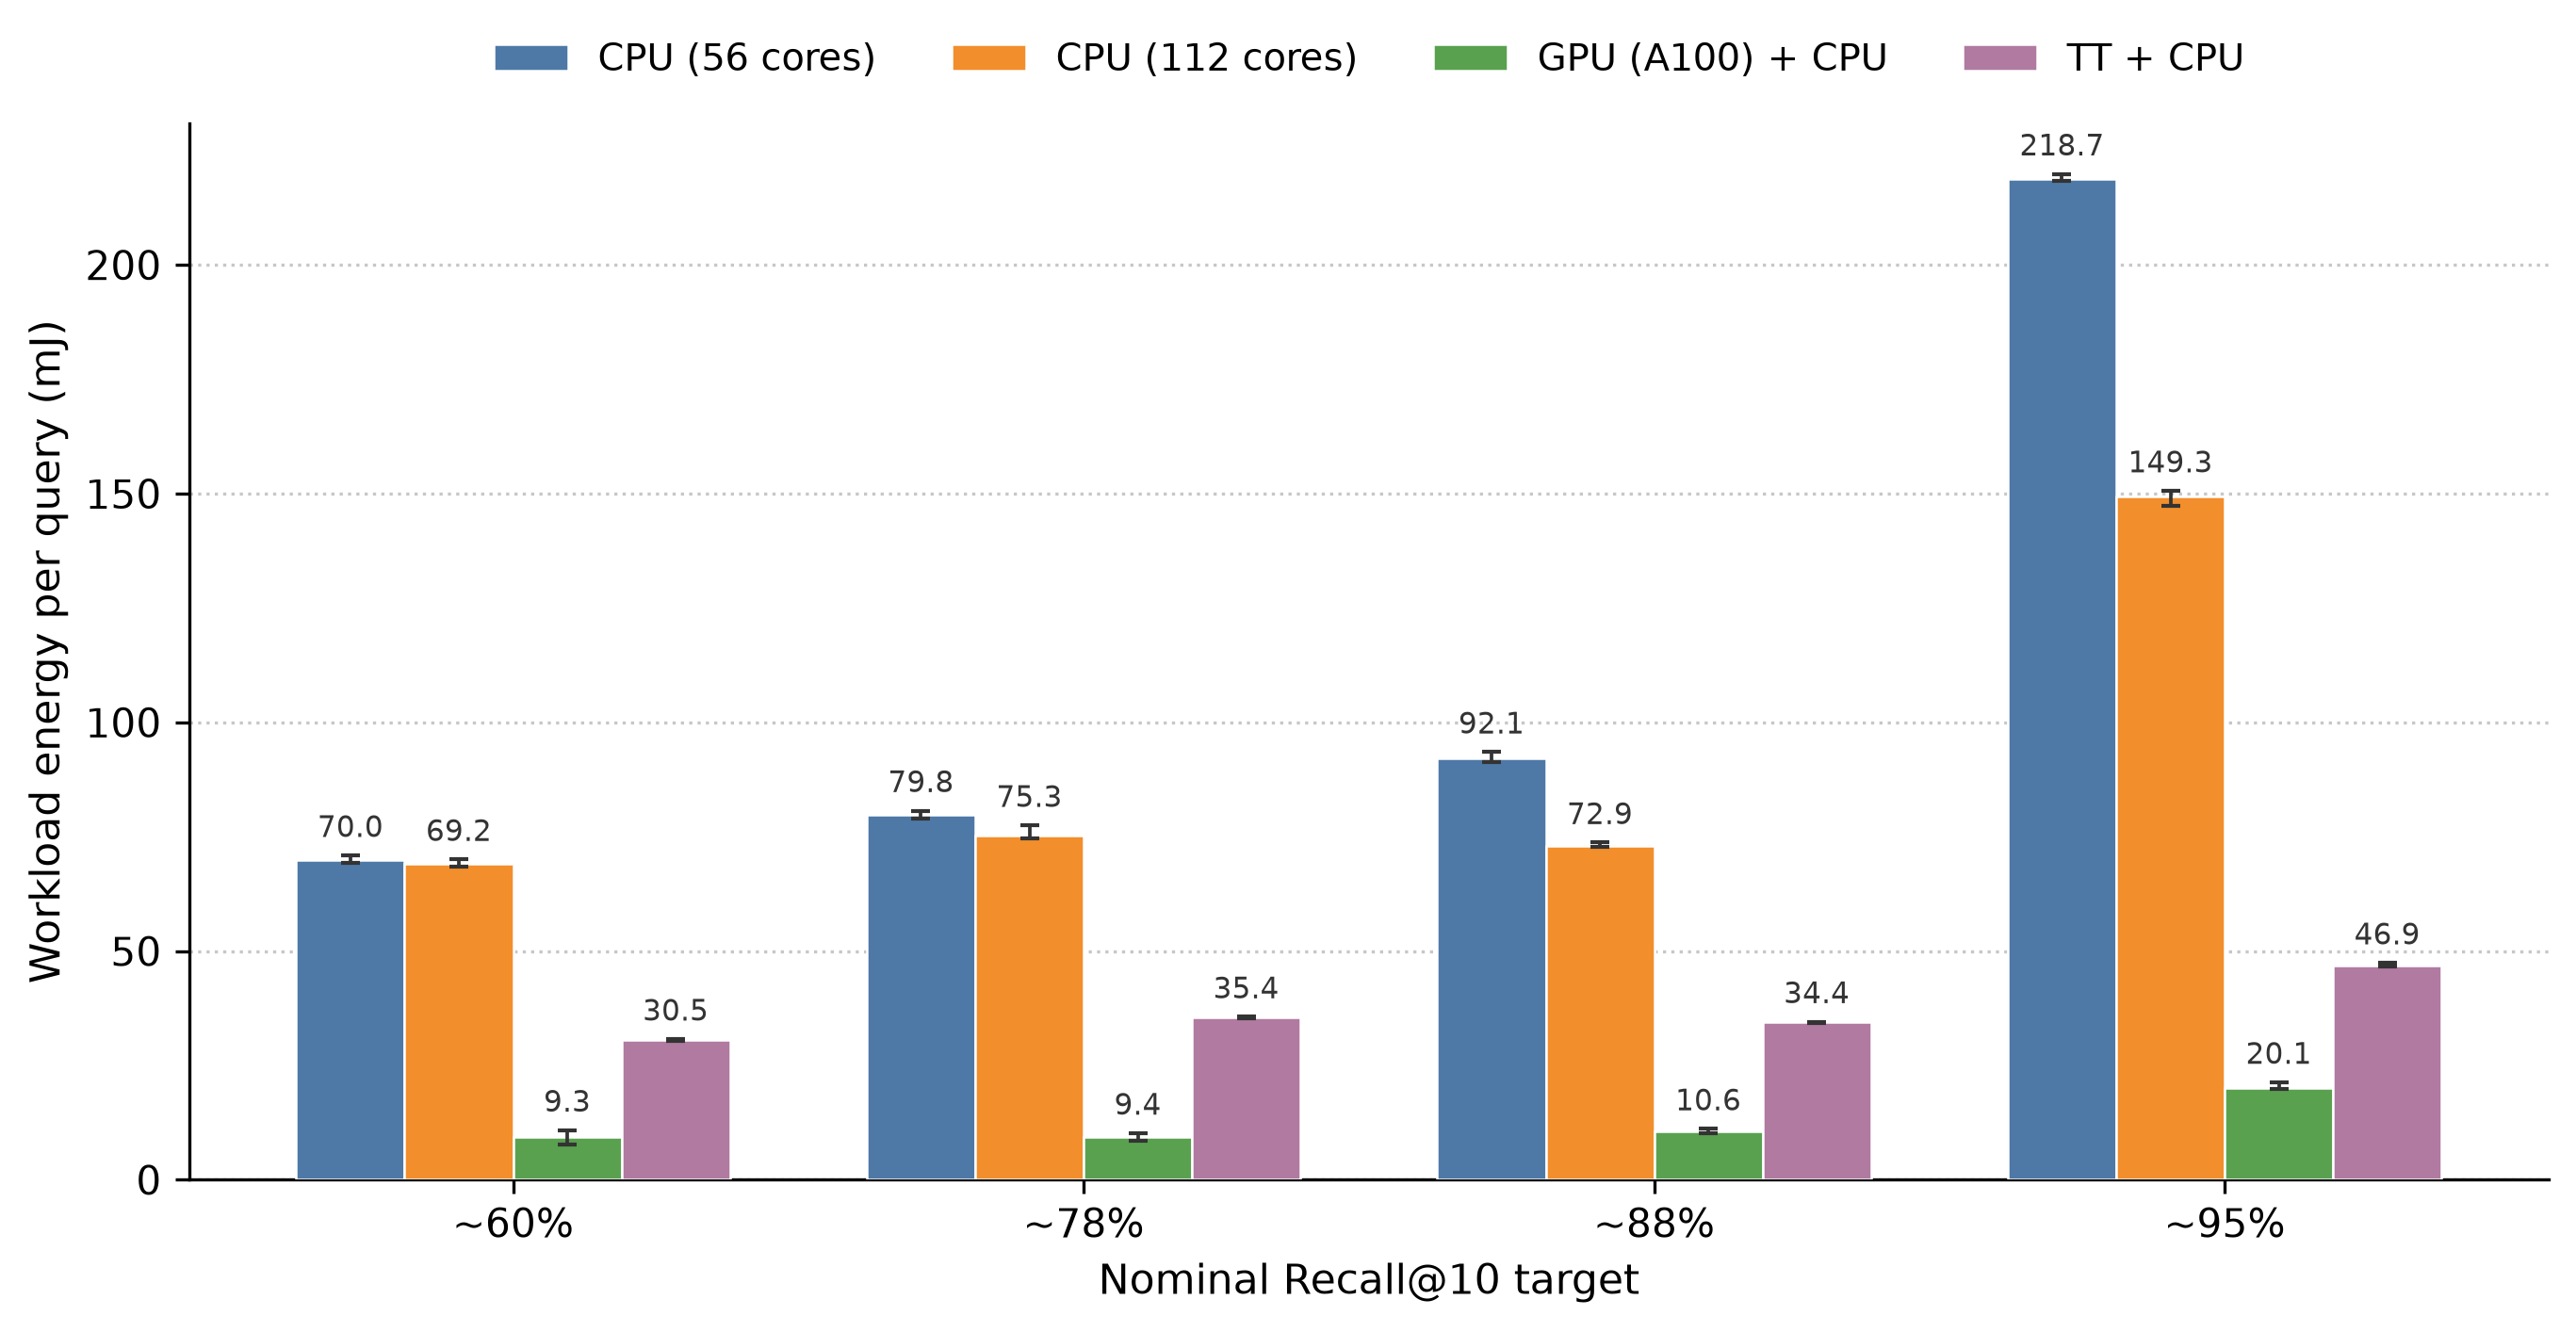
\includegraphics[width=0.96\textwidth]{./assets/energy_per_query_recall.png}
\caption{Amortized workload energy per query at approximately matched
Recall@10, including initialization. Bars show the median of ten sessions and
whiskers the interquartile range.}
\label{fig:query-energy}
\end{figure}

The GPU system uses the least energy at every target, 9.3--20.1~mJ per query.
Tenstorrent is second, with 30.5--46.9~mJ per query, which is 2.3 times the
GPU value at the 95\% target and 3.2--3.8 times at the lower targets. Both CPU
configurations use the most: 69--92~mJ per query up to the 88\% target and
149--219~mJ at 95\%. Tenstorrent therefore uses 53--63\% less energy than the
CPUs up to the 88\% target, and 78.5\% and 68.6\% less than the 56-core and
112-core CPUs at 95\%, where the GPU uses 90.8\% and 86.5\% less.

The CPU and Tenstorrent values are reproducible across sessions, with an RSD
of at most 2.67\% on the CPUs and 3.85\% on Tenstorrent. The GPU values vary more at low recall,
with an RSD of 36.6\% at 60\% and 24.0\% at 78\%, because these sessions last
less than 3~s and are almost entirely initialization; at the 88\% and 95\%
targets the RSD is about 6\%.

\paragraph{The host dominates Tenstorrent's energy.}
The Wormhole device itself uses 327--850~J per session, 23.9--33.6~W on
average, or only 10.7--18.1\% of the system energy. The remaining 152--200~W is
drawn by the dual-socket EPYC 7301 host, whose combined rated TDP of about
310--340~W is less than half that of the 700~W CPU node. The energy of the
Tenstorrent system is therefore set mainly by its host.

For a device-to-device view at the 95\% target, the A100 board trace of one
session is examined on its own; the board power is integrated in every GPU
session, but only this trace is analyzed separately here. The board draws about 66~W when idle and about 377~W
on average while searching, with a peak of 386~W, below its 550~W limit; the
high-power interval lasts 2.2~s, matching the 2.31~s search time. Over the
session the board uses 1,066~J, or 10.7~mJ per query, against 8.5~mJ for the
Wormhole chip. The two devices therefore use comparable energy for this
workload, keeping in mind that the chip telemetry of the Wormhole excludes the
board-level losses that the A100 measurement includes: the A100 draws far more
power, but finishes the search about 7.8 times faster.

The GPU system is not dominated by its host to the same extent. At the 95\%
target, the 1,066~J of the A100 board are about half of the 2,011~J median
energy of the complete A100 system, whereas the Wormhole chip accounts for only
18\% of the Tenstorrent system. Since the board figure comes from a single
session and the system figure is a median over ten, this split is approximate,
but it shows that the energy gap between the two systems lies mainly in their
host energy rather than in the accelerators. The Tenstorrent host is not more
power-hungry, drawing 152~W at this target against about 218~W for the A100
host, but it is powered for a session 5.8 times longer. The Wormhole device
thus reaches a device energy comparable to that of the A100 while being a
lower-cost accelerator, and shortening the session, through faster
initialization and search, is the most direct way to reduce the energy of the
Tenstorrent system.

\paragraph{Initialization dominates at low recall.}
Table~\ref{tab:energy-session-composition} relates each session to its search
time, estimated as \(Q_{\mathrm{run}}/\operatorname{QPS}_{\mathrm{reported}}\).
At the 60\% target, search occupies only 2--4\% of every CPU and GPU session
and 15\% of the Tenstorrent session; the remainder is process start-up,
dataset loading, list assignment, and, on the accelerators, device setup and
index transfer. The per-query values in
Table~\ref{tab:energy-recall} therefore measure the cost of a complete
100,000-query job from a cold start, not the energy of search alone.

The time spent outside search differs strongly between the platforms. On the
GPU system it is 2.0--2.8~s for every configuration. On the CPUs it grows with
\(N_{\mathrm{list}}\), from 3.0--7.2~s at 512 lists to 9.3--10.8~s at 1024 and
17.4--17.9~s at 2048, and at 1024 and 2048 lists it is almost the same on 56
and 112 cores. On
Tenstorrent, whose host also performs the assignment, it grows from 7.3~s at
512 lists to 8.2~s at 1024 and 11.6--11.7~s at 2048. This is consistent with
the assignment of the 1.18 million database vectors to their nearest
centroids, whose cost is proportional to \(N_{\mathrm{list}}\), running on the
host CPU without benefiting from additional cores, whereas the GPU performs it
on the device. The low-recall CPU and Tenstorrent energy is therefore
dominated by initialization rather than by search.

\begin{table}[htbp]
\centering
\caption{Composition of the energy sessions. Search time is
\(100{,}000/\operatorname{QPS}_{\mathrm{reported}}\); session time is the
median duration of the complete session, which includes the search; and
average power is the median workload energy divided by the median session
time.}
\label{tab:energy-session-composition}
\small
\setlength{\tabcolsep}{4pt}
\renewcommand{\arraystretch}{1.08}
\begin{tabular}{lrrrrr}
\toprule
Architecture & Target & Search (s) & Session (s) & Search share & Avg.\ power (W) \\
\midrule
CPU (56 cores)   & 60\% & 0.66  & 18.171 & 3.6\%  & 385.0 \\
                 & 78\% & 2.28  & 19.667 & 11.6\% & 405.8 \\
                 & 88\% & 8.72  & 17.983 & 48.5\% & 512.2 \\
                 & 95\% & 31.35 & 34.376 & 91.2\% & 636.3 \\
\midrule
CPU (112 cores)  & 60\% & 0.38  & 18.211 & 2.1\%  & 379.7 \\
                 & 78\% & 1.25  & 19.126 & 6.5\%  & 393.5 \\
                 & 88\% & 4.53  & 15.314 & 29.6\% & 476.2 \\
                 & 95\% & 17.18 & 24.395 & 70.4\% & 612.0 \\
\midrule
GPU (A100) + CPU & 60\% & 0.06  & 2.828  & 2.2\%  & 329.9 \\
                 & 78\% & 0.18  & 2.795  & 6.6\%  & 336.5 \\
                 & 88\% & 0.62  & 2.862  & 21.7\% & 371.8 \\
                 & 95\% & 2.31  & 4.335  & 53.3\% & 463.8 \\
\midrule
TT + CPU         & 60\% & 2.01  & 13.626 & 14.8\% & 223.8 \\
                 & 78\% & 4.56  & 16.285 & 28.0\% & 217.6 \\
                 & 88\% & 9.29  & 17.486 & 53.1\% & 196.6 \\
                 & 95\% & 18.02 & 25.294 & 71.2\% & 185.5 \\
\bottomrule
\end{tabular}
\end{table}

\paragraph{More CPU cores do not cost more energy.}
The 56-core CPU never uses less energy than the 112-core CPU. At the 60\%
target the two are within 1.2\%, because both sessions are almost entirely
initialization, which does not benefit from more cores, so the node draws about 380~W in
either configuration. As search takes a larger share of the session, the
56-core CPU uses 6\% more energy at 78\%, 26\% more at 88\%, and 47\% more at
95\%. Doubling the cores does not double the power, because most of the node's
power is fixed: both sockets, with their caches, memory controllers, and idle
cores, are powered for the whole session regardless of how many cores search.
Moreover, with 56 cores the active cores can likely run at higher clock frequencies
and draw more power each, while the idle ones still draw some; with 112 cores
all of them are active, but each draws less, so the average power changes
little.
Assuming about 380~W during initialization, the average power during the
search at the 95\% target is roughly 660~W with 56 cores and 710~W with 112,
only about 7\% more, while the search takes 31.35~s instead of 17.18~s. The
112-core search therefore spends about 12~kJ instead of 21~kJ: it pays the
fixed power of the node for a much shorter time.

\subsection{Workload Throughput and Energy}
\label{sec:session-throughput-energy}

To view speed and energy on the same workload boundary,
Figure~\ref{fig:session-throughput-energy} uses the workload throughput
\begin{equation}
\Theta_{\mathrm{workload}}
=\frac{Q_{\mathrm{run}}}{t_{\mathrm{session}}}
=\frac{100{,}000}{t_{\mathrm{session}}},
\label{eq:session-throughput}
\end{equation}
which, unlike the search-only QPS of Section~\ref{sec:cross-platform-performance},
includes initialization.

\begin{figure}[htbp]
\centering
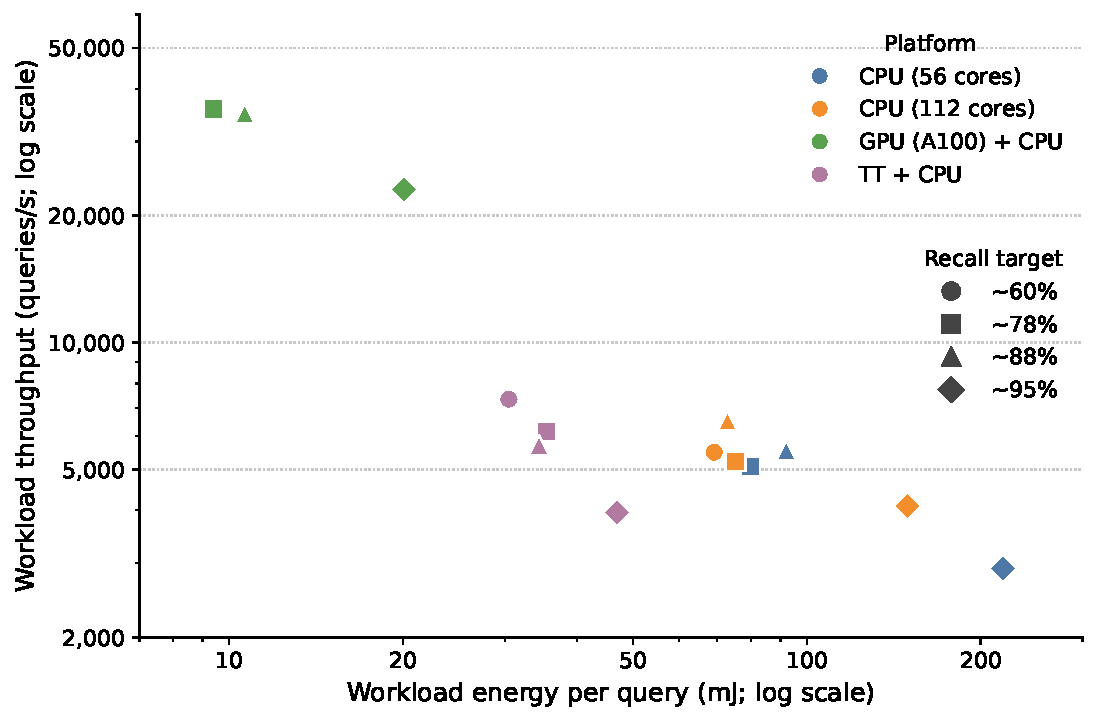
\includegraphics[width=0.94\textwidth]
{./assets/session_throughput_vs_energy.pdf}
\caption{Workload throughput, including initialization, versus amortized
workload energy per query at approximately matched Recall@10 targets.}
\label{fig:session-throughput-energy}
\end{figure}

The GPU system lies in the upper left at every target: it completes the
workload fastest, at 35,000--36,000 queries per second up to the 88\% target,
and uses the least energy. The Tenstorrent and CPU sessions reach similar
workload throughput, between about 2,900 and 7,300 queries per second, because
initialization takes a large part of each of them, but Tenstorrent uses
53--79\% less energy. At the 95\% target, the GPU, 112-core, Tenstorrent, and
56-core sessions correspond to 23,068, 4,099, 3,954, and 2,909 queries per
second. These ratios are smaller than the search-only differences in
Table~\ref{tab:qps-matched} because initialization occupies part of every
session.

\section{Summary of Results and Limitations}
\label{sec:results-summary}

The main observations are:
\begin{itemize}
    \item The GPU has the highest search throughput at every recall level, from
    31.9 times Tenstorrent at 60\% to 7.8 times at 95\%.
    \item Tenstorrent is slower than both CPU configurations up to about 88\%
    recall; at 95\% it is 1.74 times faster than the 56-core CPU and on par
    with the 112-core CPU against the evaluated Faiss grid.
    \item The batch-level union raises Tenstorrent recall by up to 7.5
    percentage points at equal parameters, but each query is scored against
    12--32 times as many vectors as in Faiss, and against 81.7\% of the
    database at the 95\% target. Consecutive queries share almost no lists. At low \(N_{\mathrm{probe}}\), Tenstorrent throughput is capped
    by a per-batch cost of about 0.58~ms.
    \item Fine search accounts for 90--98\% of the Tenstorrent search path at
    \(N_{\mathrm{list}}=512\). Inside it, reader and compute advance in
    lock-step on each list, batch transitions and aggregation are overlapped
    with worker execution, and batch completion is set by the slowest worker.
    Within a list, compute costs about 7~\(\mu\)s per page and waits for
    slow DRAM fetches for about 40\% of the time.
    \item The GPU system uses the least workload energy at every recall
    target, Tenstorrent 2.3--3.8 times as much, and the CPUs the most.
    Tenstorrent uses 53--79\% less energy than the CPUs, and its energy is
    dominated by its host, the device accounting for only 11--18\% of it. On
    the CPU node, 112 cores never use more energy than 56, because the node's
    power is drawn for the whole session and more cores finish sooner.
\end{itemize}

These results are subject to the following limitations:
\begin{itemize}
    \item \textbf{Workload boundary.} Energy includes initialization, so the
    per-query values depend on workload length and do not measure search
    energy alone.
    \item \textbf{Quality matching.} Tenstorrent and Faiss process different
    candidate sets, so cross-platform points are matched only approximately
    by recall, and the effect of alternative query groupings is not
    evaluated.
    \item \textbf{Platforms.} The three systems use different hosts and
    hardware generations, including a 2017 AMD EPYC 7301 host for
    Tenstorrent, and their device power sensors cover different parts of the
    accelerator (chip telemetry on Tenstorrent, the whole board on the A100).
    The comparison is between complete systems, not between processor
    architectures in isolation.
    \item \textbf{Dataset scale.} The 16-bit database occupies about 237~MB,
    which is small for a vector-search deployment and close to the combined
    last-level cache of the dual-socket CPU node. The dataset was chosen as a
    standard benchmark with published exact neighbors, which the
    recall-matched comparison requires. Collections of the size that
    motivates this work, such as large RAG corpora, would not fit on one
    device: in the current layout the 12~GB of the Wormhole n150 hold about
    30 million vectors (Section~\ref{sec:conclusion-limitations}); larger
    collections would require distributing the index over several devices or
    streaming lists from host memory, which are natural extensions of this
    work.
    \item \textbf{Bottleneck attribution.} The single-list trace covers 16
    pages of one list on one worker at \(N_{\mathrm{probe}}=1\). It separates fetch from compute
    but not the matrix multiplication from the top-\(k\) update, and it does
    not explain why some DRAM fetches are slow.
    \item \textbf{Quantization.} The Tenstorrent implementation uses full
    FP16 vectors with FP32 accumulation; no conclusion is drawn about 8-bit or
    other quantized fine-search paths.
\end{itemize}

\cleardoublepage
